\section{$B^- \rightarrow \bar{\Lambda_c}^-$ decays}

Applying the same procedure already illustrated in \cref{sec:chargedCorrBtoLambdaC}, the optimized selection cuts for the charged flavor-anticorrelated decays are:

\begin{itemize}
\item $foxWolframR2 < 0.3$  
 \item SignalProbability $> $ 0.1
\item $p^{\Lambda_c}_{CMS} < $ 1.5 GeV/c
\end{itemize}

\subsection{Probability Density Functions (PDFs) for the two dimensional fit}

The PDFs used to describe the signal distributions are the same already used in  \cref{sec:2DpdfChargedCorrBtoLambdaC} (only the shaping parameters differ) and an example of the 2D fit is shown in Fig. \ref{fig:stream12345_TotalSignal_charged_anticorrLambdaC_2Dfit}. Also the generic background deriving from other $B^{+}B^-$ events presents similar shapes of the distributions as shown already in  \cref{sec:2DpdfChargedCorrBtoLambdaC}, therefore the probability density functions used are the same (fit is shown in \cref{fig:streams12345_charged_anticorrLambdaC_Generic_2DFit}).

\begin{figure}[H]
\centering
{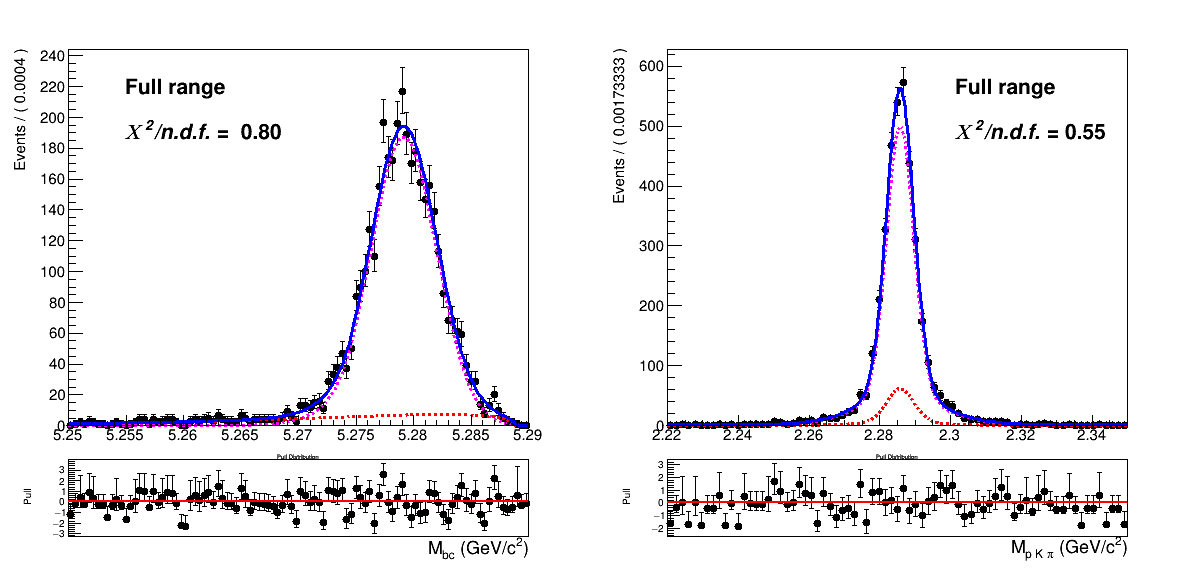
\includegraphics[width=0.75\textwidth]{06-chargedAnticorrBtoLambda/figs/stream12345_TotalSignal_charged_anticorrLambdaC_2Dfit.png}}
\caption{Two dimensional fit of total signal events in $M_{bc}$  and $M(p K \pi)$.}
\label{fig:stream12345_TotalSignal_charged_anticorrLambdaC_2Dfit}
\end{figure}

\begin{figure}[H]
\centering
{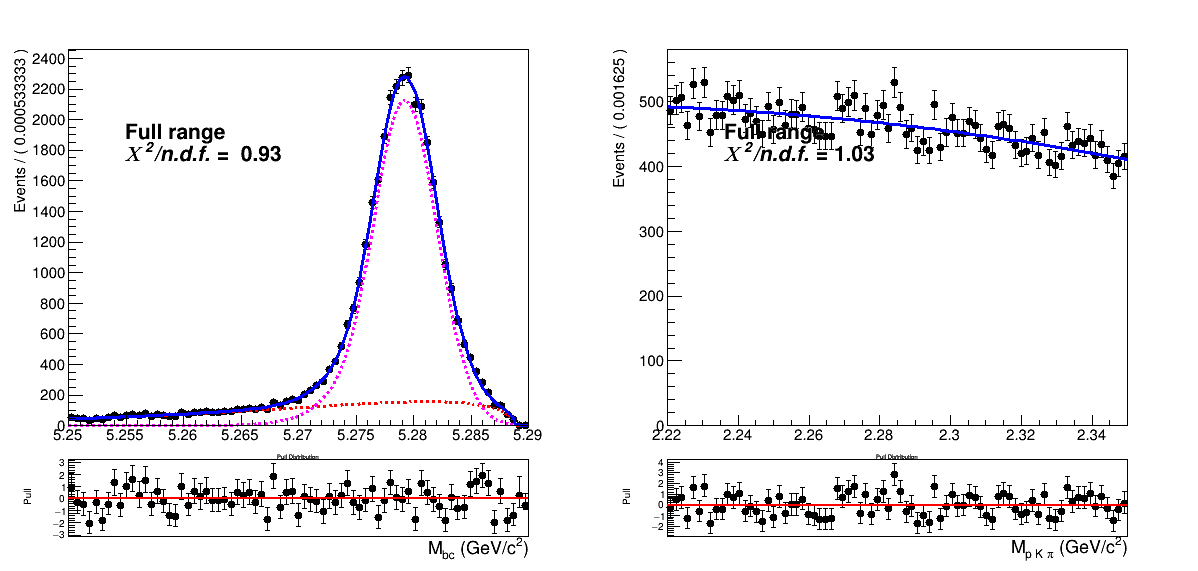
\includegraphics[width=0.75\textwidth]{06-chargedAnticorrBtoLambda/figs/streams12345_charged_anticorrLambdaC_Generic_2DFit.png}}
\caption{Two dimensional fit of generic ($B^+B^-$) events in $M_{bc}$  and $M(p K \pi)$.}
\label{fig:streams12345_charged_anticorrLambdaC_Generic_2DFit}
\end{figure}

The same can be said about the misreconstructed $B^0$ events (Fig. \ref{fig:stream12345_Crossfeed_charged_anticorrLambdaC_2Dfit})

\begin{figure}[H]
\centering
{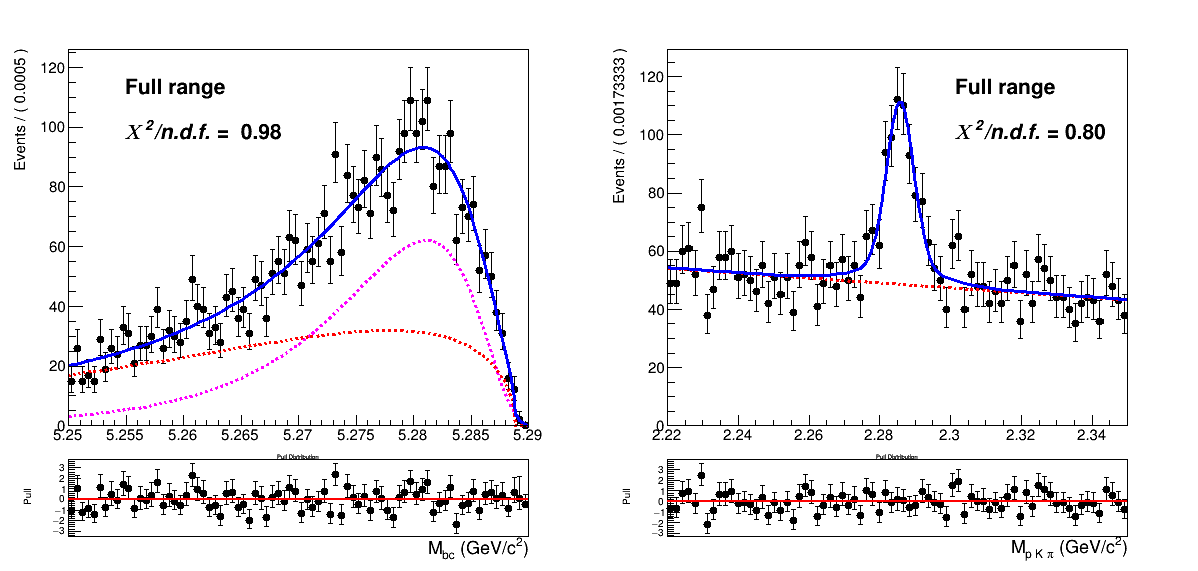
\includegraphics[width=0.75\textwidth]{06-chargedAnticorrBtoLambda/figs/stream12345_Crossfeed_charged_anticorrLambdaC_2Dfit.png}}
\caption{Two dimensional fit of crossfeed ($B^0\bar{B^0}$) events in $M_{bc}$  and $M(p K \pi)$.}
\label{fig:stream12345_Crossfeed_charged_anticorrLambdaC_2Dfit}
\end{figure}

\noindent To check that the shapes determined using 5 streams of Monte Carlo are describing with reasonable accuracy the 2D distribution, the projections of the fit of the two-dimensional distributions in the signal and sideband regions are plotted (\cref{fig:Signal_window_stream02345_Crossfeed_charged_anticorrLambdaC_2Dfit} - \cref{fig:InvM_Sideband_stream02345_Crossfeed_charged_anticorrLambdaC_2Dfit}).
One can see the same tendencies of undershooting/overshooting the $\Lambda_c$ invariant mass peak, as in the case of charged correlated decays  (Figures \ref{fig:5streams_Signal_window_Crossfeed_charged_corrLambdaC_2Dfit} - \ref{fig:5streams_Mbc_Sideband_Crossfeed_charged_corrLambdaC_2Dfit}).
But when examining the independent Monte Carlo stream distribution overlaid by the determined PDF in the very same regions (see Figures \ref{fig:Signal_window_stream1_Crossfeed_charged_anticorrLambdaC_2Dfit} -\ref{fig:Mbc_Sideband_stream1_Crossfeed_charged_anticorrLambdaC_2Dfit})
those effects are so much diminished, according to the statistics, that the effects are within statistical fluctuations and therefore negligible, contrary to the case of charged flavor-correlated decays.


\begin{figure}[H]
\centering
{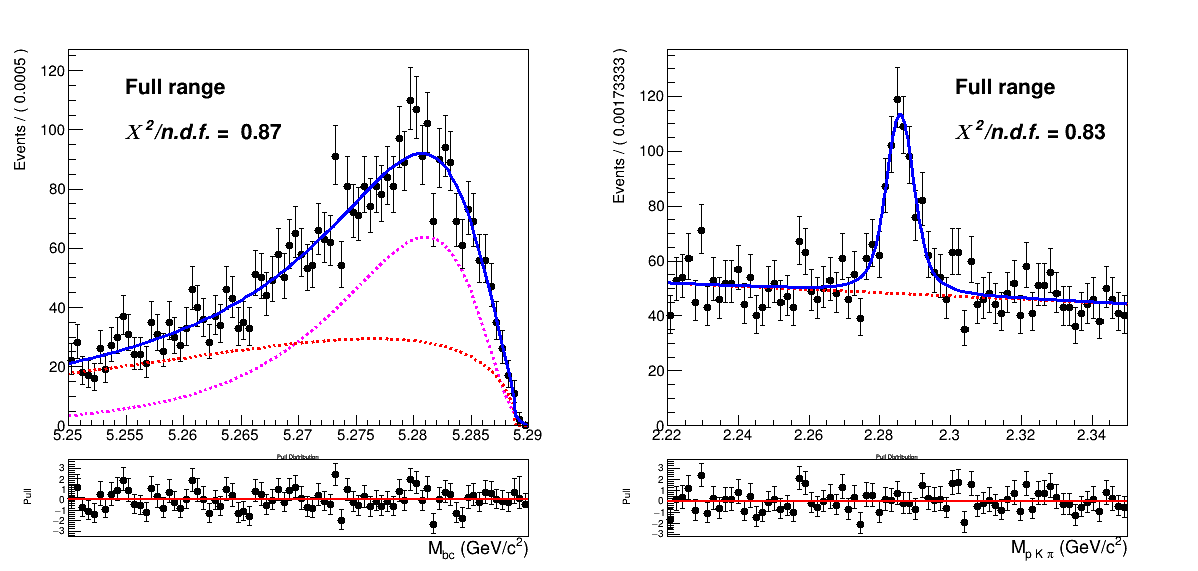
\includegraphics[width=0.75\textwidth]{06-chargedAnticorrBtoLambda/figs/stream02345_Crossfeed_charged_anticorrLambdaC_2Dfit.png}}
\caption{Two dimensional fit of crossfeed ($B^0\bar{B^0}$) events in $M_{bc}$  and $M(p K \pi)$.}
\label{fig:stream02345_Crossfeed_charged_anticorrLambdaC_2Dfit}
\end{figure}


\begin{figure}[H]
\centering
{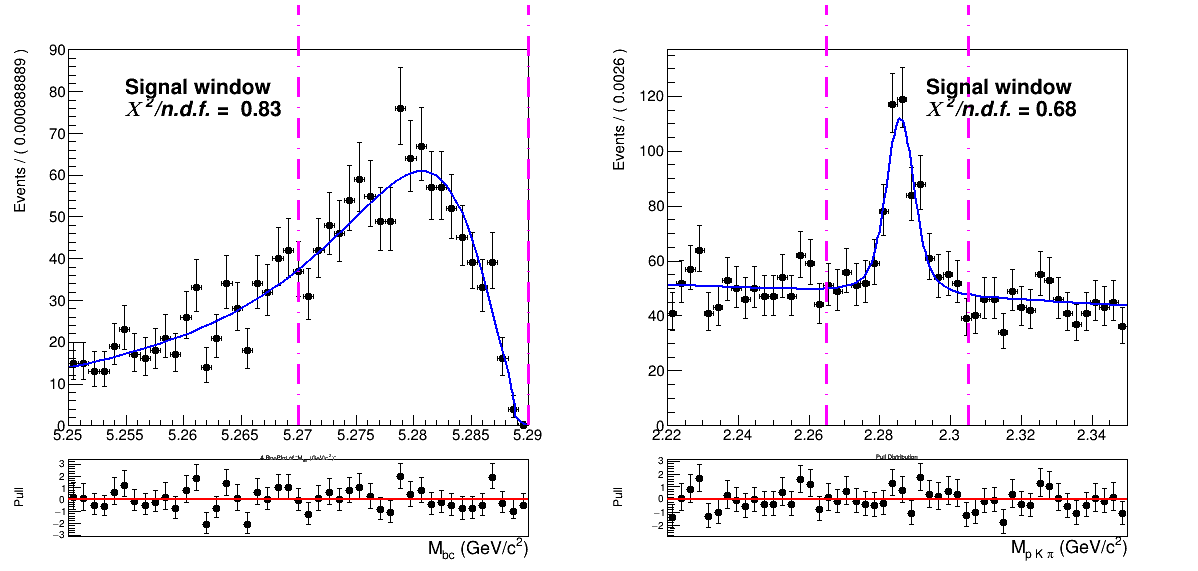
\includegraphics[width=0.75\textwidth]{06-chargedAnticorrBtoLambda/figs/Signal_window_stream02345_Crossfeed_charged_anticorrLambdaC_2Dfit.png}}
\caption{Signal region projections in $M_{bc}$ and $M(p K \pi)$  of the fit of crossfeed events.}
\label{fig:Signal_window_stream02345_Crossfeed_charged_anticorrLambdaC_2Dfit}
\end{figure}

\begin{figure}[H]
\centering
{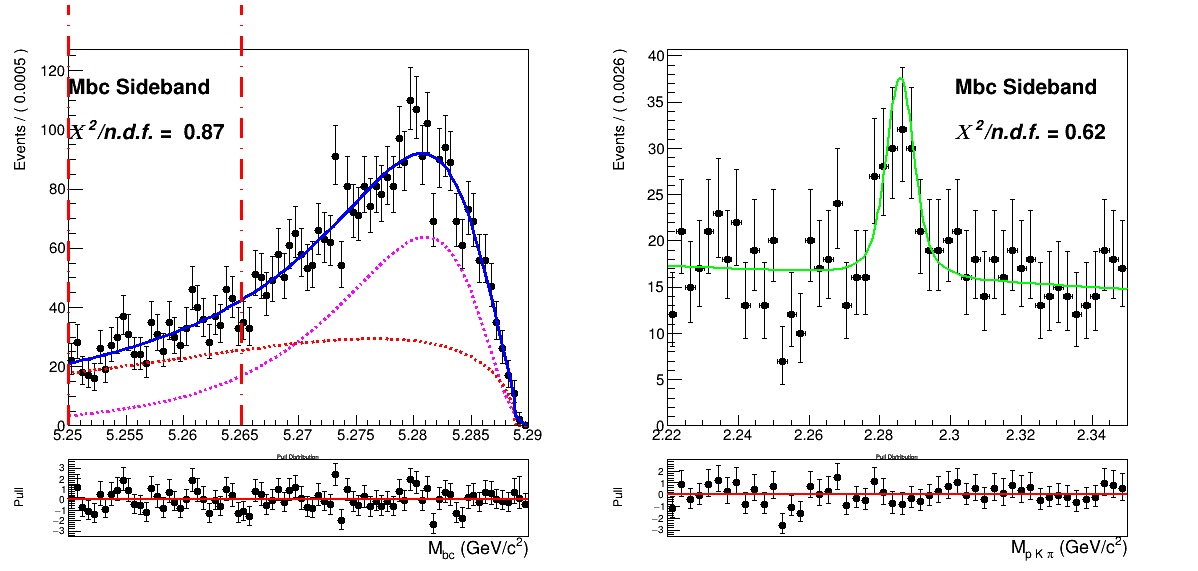
\includegraphics[width=0.75\textwidth]{06-chargedAnticorrBtoLambda/figs/Mbc_Sideband_stream02345_Crossfeed_charged_anticorrLambdaC_2Dfit.png}}
\caption{$M_{bc}$ sideband region projection of the fit of crossfeed events in $M(p K \pi)$.}
\label{fig:Mbc_Sideband_stream02345_Crossfeed_charged_anticorrLambdaC_2Dfit}
\end{figure}



\begin{figure}[H]
\centering
{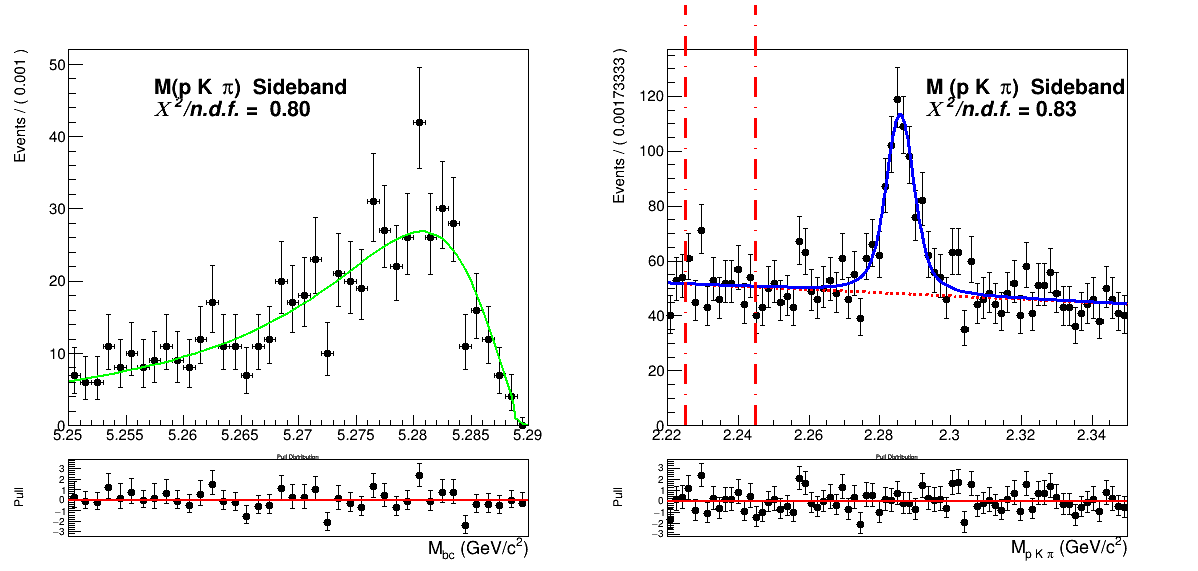
\includegraphics[width=0.75\textwidth]{06-chargedAnticorrBtoLambda/figs/InvM_Sideband_stream02345_Crossfeed_charged_anticorrLambdaC_2Dfit.png}}
\caption{$M(p K \pi)$ sideband region projection of the fit of crossfeed events in $M_{bc}$.}
\label{fig:InvM_Sideband_stream02345_Crossfeed_charged_anticorrLambdaC_2Dfit}
\end{figure}




\begin{figure}[H]
\centering
{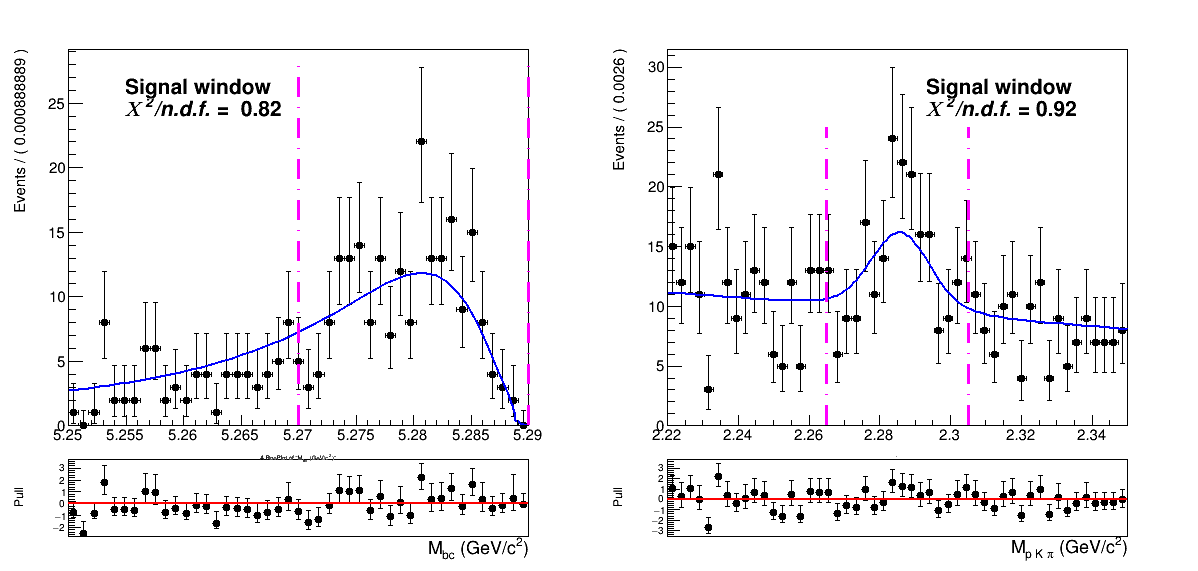
\includegraphics[width=0.75\textwidth]{06-chargedAnticorrBtoLambda/figs/Signal_window_stream1_Crossfeed_charged_anticorrLambdaC_2Dfit.png}}
\caption{Signal region projections in $M_{bc}$ and $M(p K \pi)$  of the fit of crossfeed events.}
\label{fig:Signal_window_stream1_Crossfeed_charged_anticorrLambdaC_2Dfit}
\end{figure}


\begin{figure}[H]
\centering
{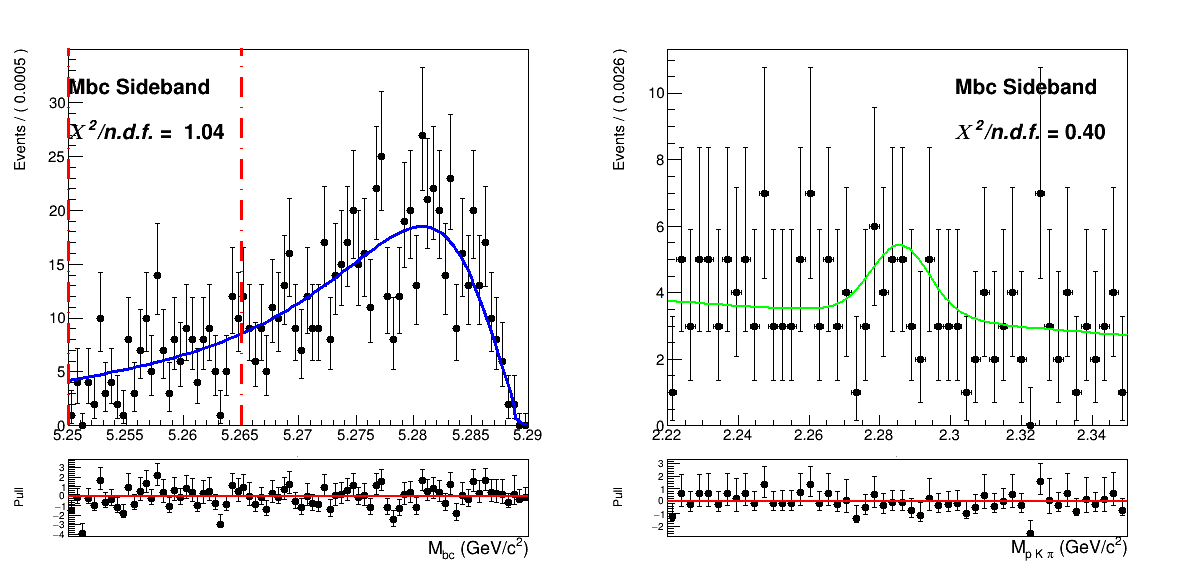
\includegraphics[width=0.75\textwidth]{06-chargedAnticorrBtoLambda/figs/Mbc_Sideband_stream1_Crossfeed_charged_anticorrLambdaC_2Dfit.png}}
\caption{Two dimensional fit of crossfeed ($B^0\bar{B^0}$) events in $M_{bc}$  and $M(p K \pi)$.}
\label{fig:Mbc_Sideband_stream1_Crossfeed_charged_anticorrLambdaC_2Dfit}
\end{figure}

\begin{figure}[H]
\centering
{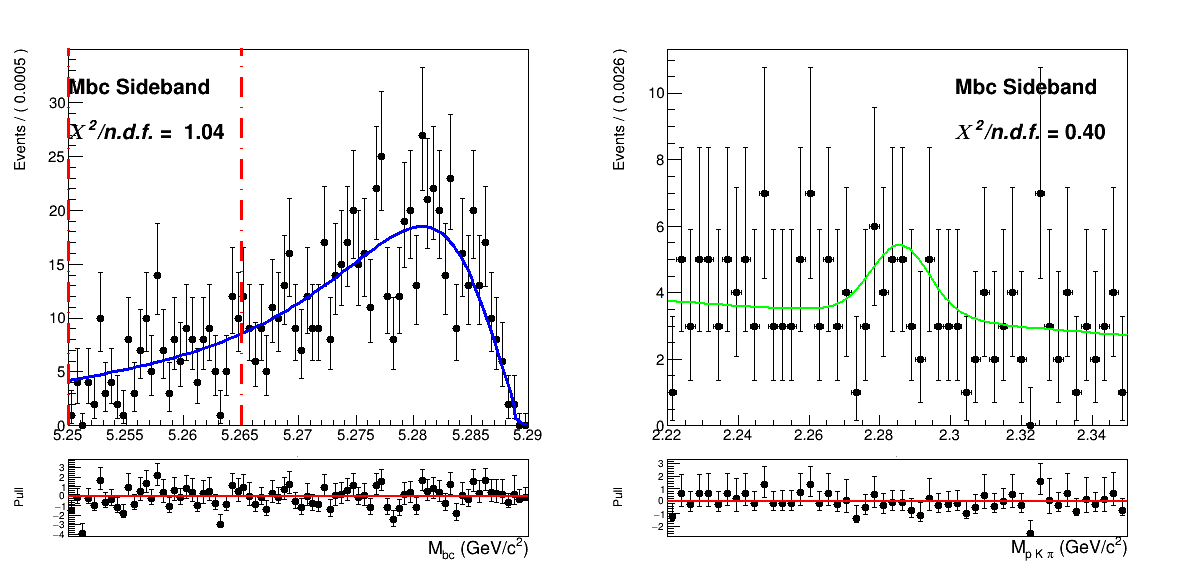
\includegraphics[width=0.75\textwidth]{06-chargedAnticorrBtoLambda/figs/Mbc_Sideband_stream1_Crossfeed_charged_anticorrLambdaC_2Dfit.png}}
\caption{Two dimensional fit of crossfeed ($B^0\bar{B^0}$) events in $M_{bc}$  and $M(p K \pi)$.}
\label{fig:Mbc_Sideband_stream1_Crossfeed_charged_anticorrLambdaC_2Dfit}
\end{figure}


\begin{figure}[H]
\centering
{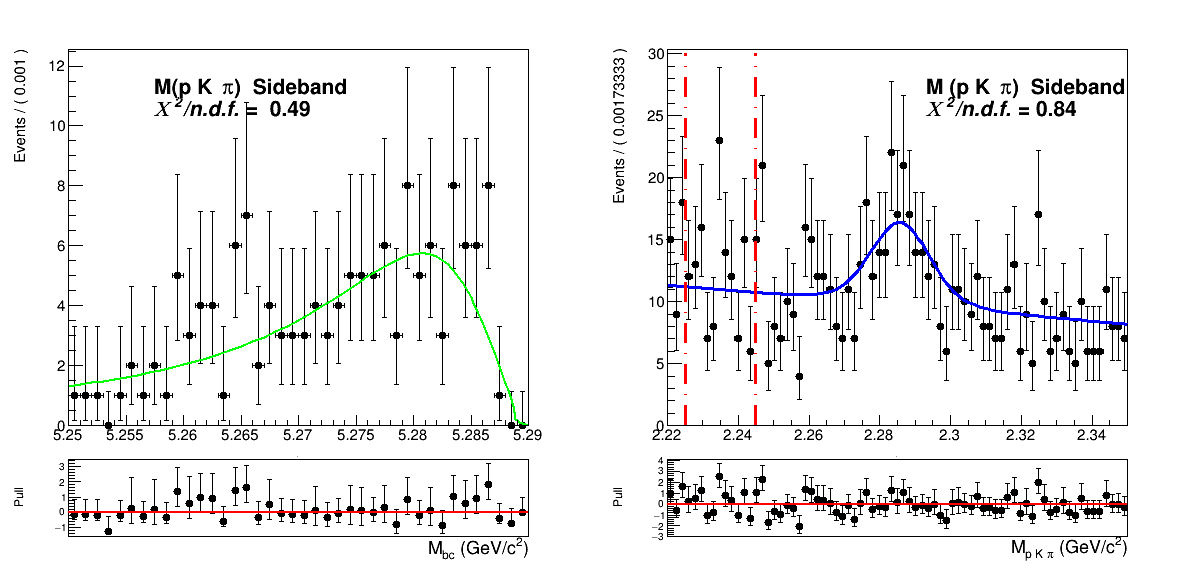
\includegraphics[width=0.75\textwidth]{06-chargedAnticorrBtoLambda/figs/InvM_Sideband_stream1_Crossfeed_charged_anticorrLambdaC_2Dfit.png}}
\caption{Two dimensional fit of crossfeed ($B^0\bar{B^0}$) events in $M_{bc}$  and $M(p K \pi)$.}
\label{fig:InvM_Sideband_stream1_Crossfeed_charged_anticorrLambdaC_2Dfit}
\end{figure}


\vspace{2.5 cm}

\noindent  The procedure adopted to model the continuum background is the same used for the charged correlated $B \rightarrow \Lambda_c$ decays. To obtain the shape that can describe the continuum background  $M_{bc}$ distribution, the continuum suppression is not applied on the off-resonance continuum sample in order to acquire more statistics. It is then scaled and corrected for the \textit{SignalProbability} correlated effects. The scaling and bin-correction procedure was carried out on a sample of five streams of on- and off-resonance MC. From a ratio plot, like the one in Fig. \ref{fig:stream02345_charged_anticorrLambdaC_woCScuts_Mbc_scaling}, showing the continuum on-resonance distribution in $M_{bc}$ and the scaled continuum on-resonance distribution without the continuum suppression applied, the bin-correction is obtained to correct the off-resonance data in the scaling procedure. The validity of this procedure is first tested on the sixth independent MC sample:      
Fig. \ref{fig:MC_on_off_resonance_stream2_anticorrLambda_continuum_2D_Mbc_corrected} shows the scaled and bin-corrected off-resonance continuum histogram compared with the continuum on-resonance distribution of the independent stream. 
Compared to the charged correlated decays one can notice larger statistical fluctuations but the overall result looks still fairly reasonable. In order to obtain the PDF describing the distribution the histogram is fitted (see Fig. \ref{fig:stream2_rescaledMbc_40binsHist_Novosibirsk}), i.e. with a Novosibirsk function. \\
Since in the $\Lambda_c$ invariant mass one doesn't expect correlation effects, one can fit directly the properly scaled distribution with a first order polynomial (see Fig.\ref{fig:stream02345_anticorrLambdaC_total_continuum_InvM_Fit_off})
\noindent It is possible then to check the validity of the whole procedure on the on-resonance Monte Carlo independent stream (Fig. \ref{fig:stream1_anticorrLambddaC_total_continuum_2DFit_Novosibirsk})  


\begin{figure}[H]
\centering
\subcaptionbox{\label{fig:stream02345_charged_anticorrLambdaC_woCScuts_Mbc_scaling}}
{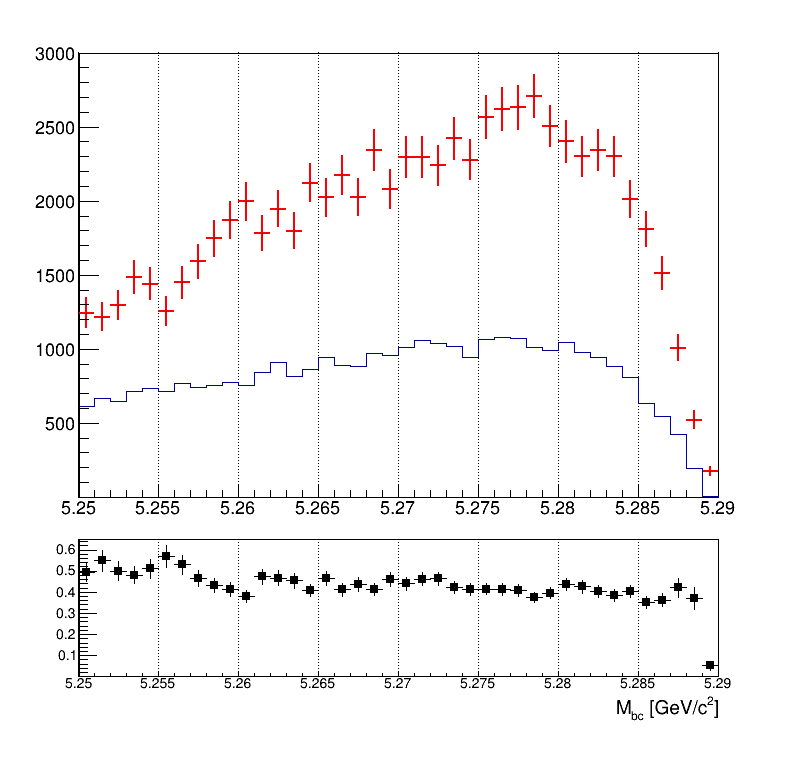
\includegraphics[width=.45\textwidth]{06-chargedAnticorrBtoLambda/figs/stream02345_charged_anticorrLambdaC_woCScuts_Mbc_scaling.png}} \quad
\subcaptionbox{\label{fig:MC_on_off_resonance_stream2_anticorrLambda_continuum_2D_Mbc_corrected}}
{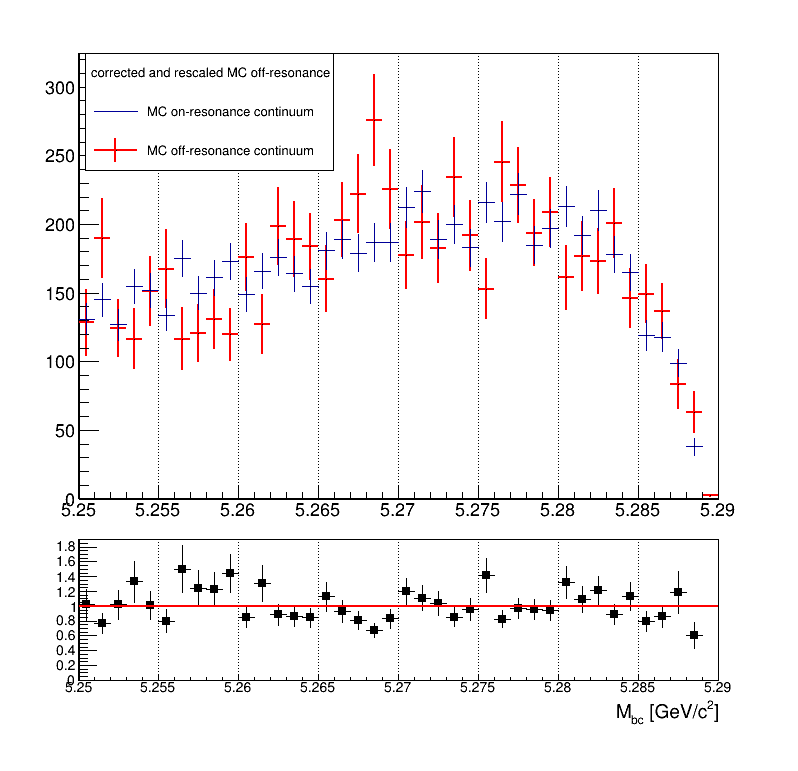
\includegraphics[width=.45\textwidth]{06-chargedAnticorrBtoLambda/figs/MC_on_off_resonance_stream2_anticorrLambda_continuum_2D_Mbc_corrected.png}} \quad
\caption{On the left: $M_{bc}$ distributions of the MC off-resonance sample without continuum suppression and the MC continuum sample with applied continuum suppression (5 streams). On the right: $M_{bc}$ distributions of the corrected scaled MC off-resonance and on-resonance MC continuum (independent stream).}
\end{figure}


\begin{figure}[H]
\centering
\subcaptionbox{\label{fig:stream2_rescaledMbc_40binsHist_Novosibirsk}}
{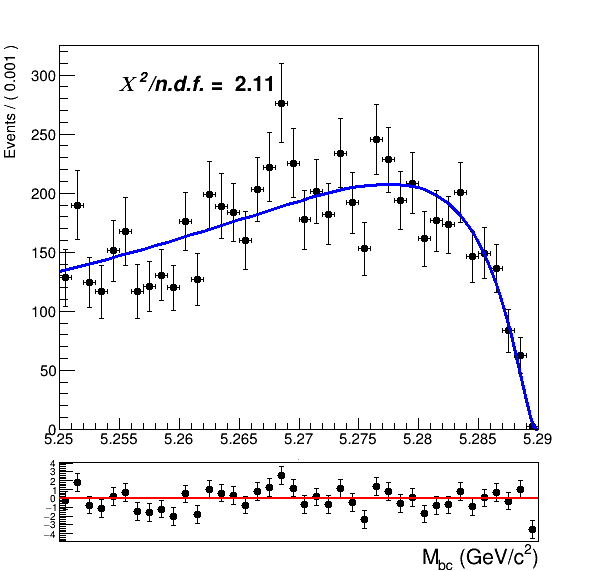
\includegraphics[width=0.45\textwidth]{06-chargedAnticorrBtoLambda/figs/stream2_rescaledMbc_40binsHist_Novosibirsk.png}} \quad
\subcaptionbox{\label{fig:stream02345_anticorrLambdaC_total_continuum_InvM_Fit_off}}
{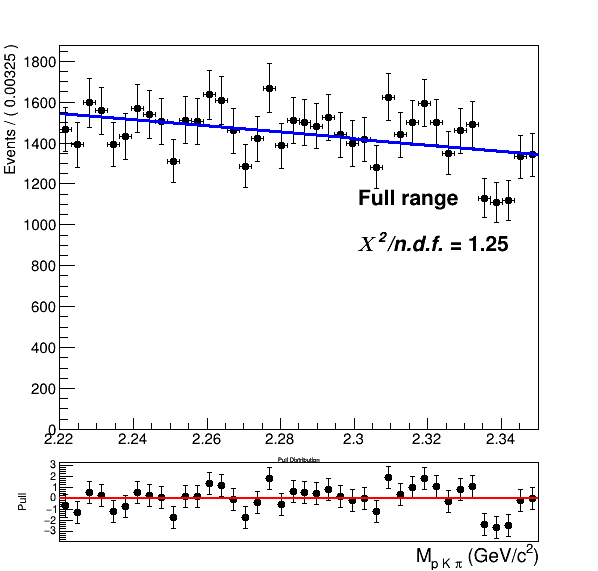
\includegraphics[width=.45\textwidth]{06-chargedAnticorrBtoLambda/figs/stream02345_anticorrLambdaC_total_continuum_InvM_Fit_off-resonance.png}} \quad
\caption{On the left: fit of the $M_{bc}$ distribution MC (scaled and corrected) off-resonance continuum (one stream). On the right: fit of the $\Lambda_c$ invariant mass distribution of five stream scaled off-resonance continuum.}
%\label{fig:stream2_rescaledMbc_40binsHist_Novosibirsk}
\end{figure}


\begin{figure}[H]
\centering
{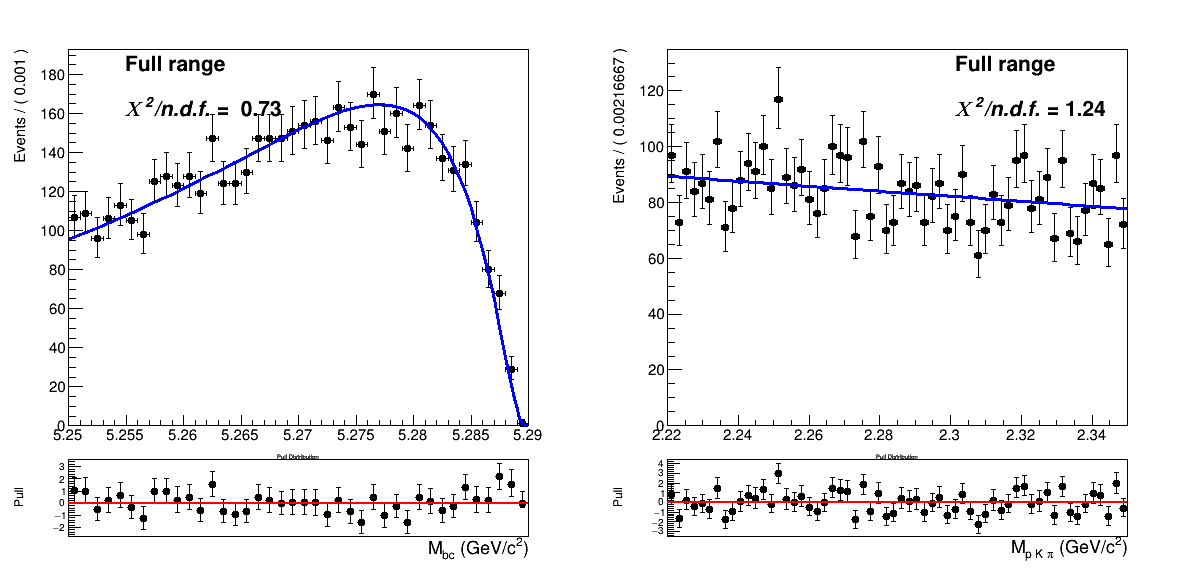
\includegraphics[width=0.85\textwidth]{06-chargedAnticorrBtoLambda/figs/stream1_anticorrLambddaC_total_continuum_2DFit_Novosibirsk.png}}
\caption{Continuum $M_{bc}$  and $M(p K \pi)$ distributions overlaid by the PDFs obtained in fits shown in Figures \ref{fig:stream2_rescaledMbc_40binsHist_Novosibirsk} - \ref{fig:stream02345_anticorrLambdaC_total_continuum_InvM_Fit_off}}
\label{fig:stream1_anticorrLambddaC_total_continuum_2DFit_Novosibirsk}
\end{figure}

\subsection{Two dimensional fit}\label{sec:chargedAnticorr2DtotalFit}
After obtaining the PDFs describing the various signal/background components using five streams statistics, the fit model is tested with six fits on the six independent Monte Carlo streams. The conditions for these six two dimensional fits are again the same used for the charged correlated decays (see Sec. \ref{2DtotalFit}).
\noindent Exemplary, the distributions of stream 0 overlaid by the fitted PDF are depicted in Fig. \ref{fig:Total_2DFit_stream0_chargedAnticorrLambdaC_Crossfeed_fraction} (see \cref{sec:chargedAnticorrApp}                       
for the projections in signal and sideband regions). 
In Table \ref{tab:SixStreams_chargedCorrLam2Dfits} the signal yields of the fits (\textbf{Reconstructed Signal}) to the two dimensional distributions for the six streams of $B^- \rightarrow \bar{\Lambda_c}^-$ flavor-anticorrelated decays are listed and compared to the expected yields of reconstructed signal, and fitted and truth-matched total signal events are also compared, together with their deviations.

\begin{figure}[H]
\centering
{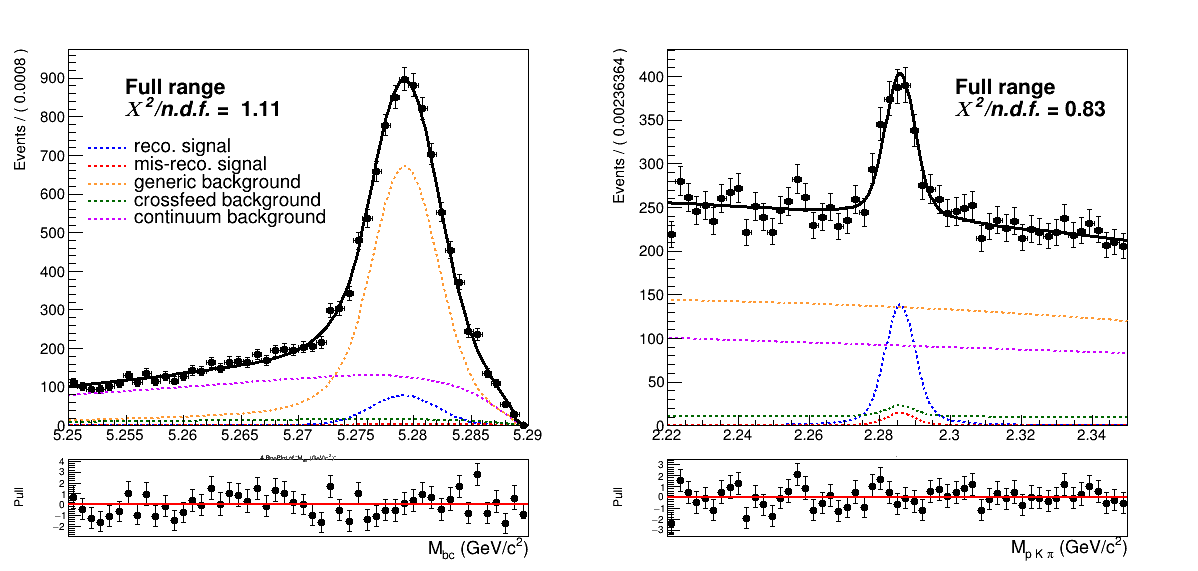
\includegraphics[width=0.85\textwidth]{06-chargedAnticorrBtoLambda/figs/Total_2DFit_stream0_chargedAnticorrLambdaC_Crossfeed_fraction_parametrization.png}}
\caption{Two dimensional fit on stream 0 Monte Carlo simulated data.}
\label{fig:Total_2DFit_stream0_chargedAnticorrLambdaC_Crossfeed_fraction}
\end{figure}

\begin{table}[h]
\centering
\resizebox{0.8\textwidth}{!}{%
\setlength{\tabcolsep}{8pt}
\begin{tabular}{c c c c c c c}

\toprule
 \hline
   &	\multicolumn{2}{c}{Reconstructed Signal}  & \multicolumn{2}{c}{Total Signal} &  \\
     &  fit \hspace{0.5 cm}  & expected  & fit   & MC truth &  \multicolumn{2}{c}{fit - MC truth} \\
 \midrule
 \hline
stream 0	&	730 $\pm$ 60 	&	660 $\pm$ 21	&	805 $\pm$ 65	&	765	&  40	&	5.2 $\%$	\\
stream 1	&	732 $\pm$ 60	&	698 $\pm$ 29	&	794 $\pm$ 63	&	785	&  9	&	1.1$\%$	\\
stream 2	&	759 $\pm$ 65	&	718 $\pm$ 29	&	800 $\pm$ 67	&	797	& 3	&	0.4$\%$	\\
stream 3	&	725 $\pm$ 58	&	702 $\pm$ 29	&	769 $\pm$ 60	&	802	& -33	&	-4.1$\%$	\\
stream 4	&	829 $\pm$ 67	&	710 $\pm$ 29	&	944 $\pm$ 76	&	804	& 140  	&	17.4$\%$	\\
stream 5	&	650 $\pm$ 61	&	675 $\pm$ 29	&	703 $\pm$ 62	&	760	&  -57	&	-8.1$\%$	\\
\midrule
\hline
sum			&	4425		&	4163	&		4815		&	4718	&	102	&	+ 2.2$\%$	\\
\bottomrule
\hline
\end{tabular}%
}%
\caption{Comparison of fitted and expected signal yields, fitted and truth-matched total signal for six streams of Belle generic MC when fitting the two dimensional distributions of $M_{bc}$ and $M(p K \pi)$.}
\label{tab:SixStreams_chargedAnticorrLam2Dfits}
\end{table}

\noindent Except for stream 4 all the fits show values of reconstructed signal within the 1$\sigma$ uncertainties in agreement with the expected ones, 
but as already encountered in Sec. \ref{2DtotalFit} a tendency of overestimation can be seen also in these fits, confirmed by the fit shown in Fig \ref{fig:RecoSignal_streams_fittedPoints_charged_anticorrLambdaC}. Again this small, but not negligible, bias has to  be taken into account while fitting the data.


\begin{figure}[H]
\centering
{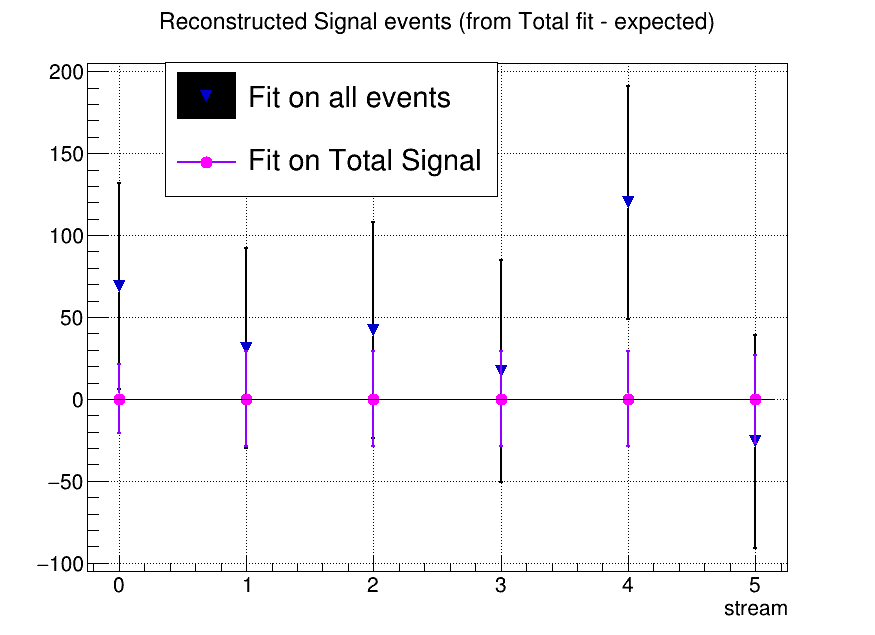
\includegraphics[width=0.75\textwidth]{06-chargedAnticorrBtoLambda/figs/Fitted_RecoSignal_chargedAntiCorrLambdaC.png}}
\caption{Differences between results from the fits and "expected" values for signal yields as reported in the first columns on Table \ref{tab:SixStreams_chargedAnticorrLam2Dfits} .}
\label{fig:chargedAnticorrRecoSignal_fit-expectedPlot}
\end{figure}

\begin{figure}[H]
\centering
{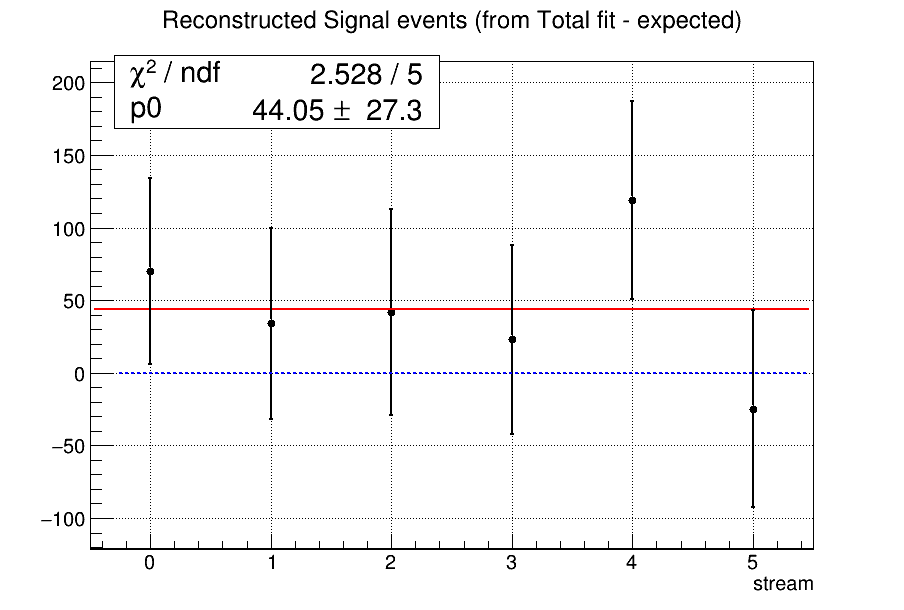
\includegraphics[width=0.85\textwidth]{06-chargedAnticorrBtoLambda/figs/RecoSignal_streams_fittedPoints_chargedAnticorrLambdaC_w_CrossfeedRatio_param.png}}
\caption{}
\label{fig:RecoSignal_streams_fittedPoints_charged_anticorrLambdaC}
\end{figure}

\noindent  Also the behaviour for different signal-to-background ratio was investigated using the six independent streams of continuum and all the ten independent streams of $B\bar{B}$ events for the generic and crossfeed backgrounds and for the signal events. 
The amount of total signal is varied between 50$\%$ and 275$\%$ of the nominal (MC) values, in order to cover the values spanned by the uncertainties on the measurement perfromed by $BaBar$ ($\mathcal{B}(B^+ \rightarrow \bar{\Lambda}_c^+ X) = 2.1^{+0.9}_{-0.6} $)
 and even the values covered by twice larger uncertainties as one can see in \cref{fig:Charged_anticorrLambda_BR_LinearityTest}. 
The values seem to distribute according to a linear dependence,  therefore also for this decay channel one doesn't expect any systematics due to different signal-to-background ratio.% The linear fit suggests a compatibility with a 1:1 relation: the red and the blue dotted lines don't overlap, but the values of the fitted line are compatible within the uncertainties with the identity line. Though also in this second test we see a slight tendency of overshooting the expected values.   


\begin{figure}[H]
%\centering
{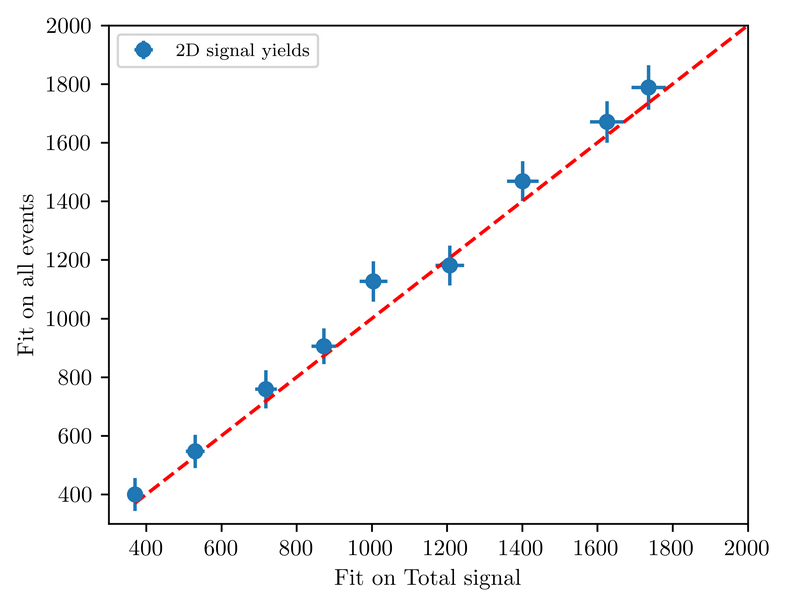
\includegraphics[width=0.75\textwidth]{06-chargedAnticorrBtoLambda/figs/Charged_anticorrLambda_LinearityTest.png}}
\caption{Linearity test: on the x-axis the obtained reconstructed signal yields from fits on different amounts of total signal; on y-axis the yields of reconstructed signal obtained fitting all events
 (as in Fig. \ref{fig:stream0_Total2Dfit_charged_corrLambdaC}). The dashed red line represents the 1:1 linear dependence.}
\label{fig:Charged_anticorrLambda_LinearityTest}
\end{figure}



\begin{figure}[H]  
  %\centering
{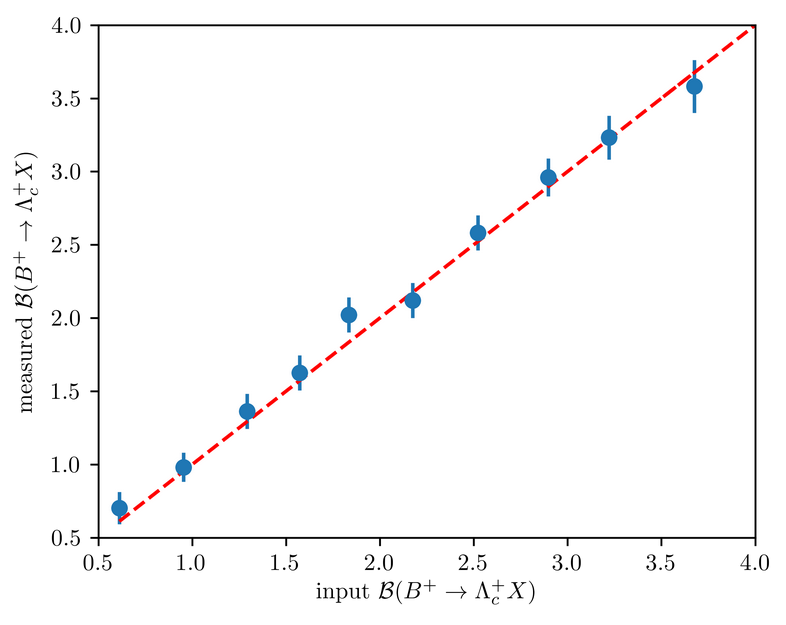
\includegraphics[width=0.75\textwidth]{06-chargedAnticorrBtoLambda/figs/Charged_anticorrLambda_BR_LinearityTest.png}}
\caption{Linearity test: on the x-axis the input branching ratio value corresponding to the signal yields displayed on the x-axis in \cref{fig:Charged_anticorrLambda_LinearityTest}; 
on y-axis the measured branching fraction values corresponding to the signal yields of reconstructed signal displayed on the y-axis in \cref{fig:Charged_anticorrLambda_LinearityTest}.}
\label{fig:Charged_anticorrLambda_BR_LinearityTest}
\end{figure}

\noindent  Toy MC pseudo-experiments were performed as well (see Appendix).%, which also don't show evidence of any bias on the signal yields. 
 
\newpage

\subsection{Probability Density Functions (PDFs) for the $B_{tag}$}
The $M_{bc}$ distribution of the tagged  $B$ mesons is fitted with a Crystal Ball as for the "peaking" component and the "flat" component is fitted with a Argus function (Fig. \ref{fig:stream0_anticorr_chargedBtag_Total_Signal_fit}).
The crossfeed background, consisting of neutral $B$ mesons tagged as charged $B$, is fitted instead with a sum of a Novosibirsk and an asymmetric Gaussian PDF (Fig. \ref{fig:NeutralCrossfeed_stream0_anticorrLambdaC_chargedBtag_MbcFit}).


\begin{figure}[H]
\begin{minipage}{.5\textwidth}
\centering
\subcaptionbox{\label{fig:stream0_anticorr_chargedBtag_Total_Signal_fit}}
{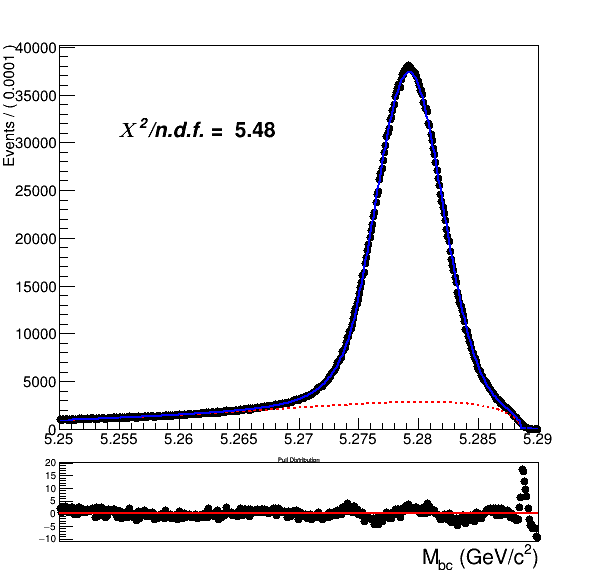
\includegraphics[width=0.80\textwidth]{06-chargedAnticorrBtoLambda/figs/stream0_anticorr_chargedBtag_Total_Signal_fit.png}}
\end{minipage} 
 \begin{minipage}{.5\textwidth}
\subcaptionbox{\label{fig:NeutralCrossfeed_stream0_anticorrLambdaC_chargedBtag_MbcFit}}
{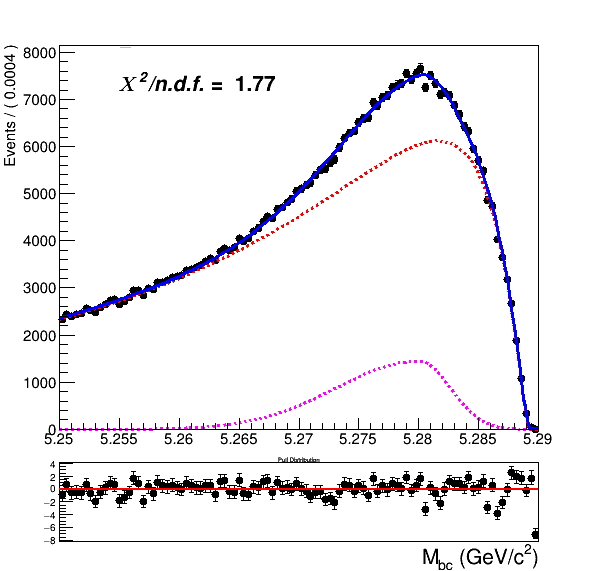
\includegraphics[width=0.80\textwidth]{06-chargedAnticorrBtoLambda/figs/NeutralCrossfeed_stream0_anticorrLambdaC_chargedBtag_MbcFit.png}}
\end{minipage}
\caption{On the left: fitted distribution of tagged charged $B$ mesons, reconstructed signal events (magenta) are described by a Crystal Ball whereas the misreconstructed signal events (red) are described by an Argus function. On the right: Crossfeed distribution fitted with a sum of Novosibirsk (red) and asymmetric Gaussian PDF (magenta)}
\end{figure}


\vspace{0.25 cm}

\noindent As for the continuum background, same procedure as the one in the case of charged flavor-correlated decays is adopted:

\begin{itemize}
    \item first the off-resonance sample is scaled accordingly with all the included cuts.
    \item the ratio between the scaled off-resonance and the on-resonance in MC is calculated in each bin (see Fig. \ref{fig:stream0_chargedAnticorrBtag_off-on_resonance})
    \item the bin-correction is applied on an independent stream and the scaled and bin-corrected $M_{bc}$ distribution is compared with the on-resonance distribution as shown in Fig. \ref{fig:stream1_chargedB_anticorrLambdaCoffresonance_scaled_check}
\end{itemize}

\begin{figure}[H]
 \centering
\subcaptionbox{\label{fig:stream0_chargedAnticorrBtag_off-on_resonance}}
{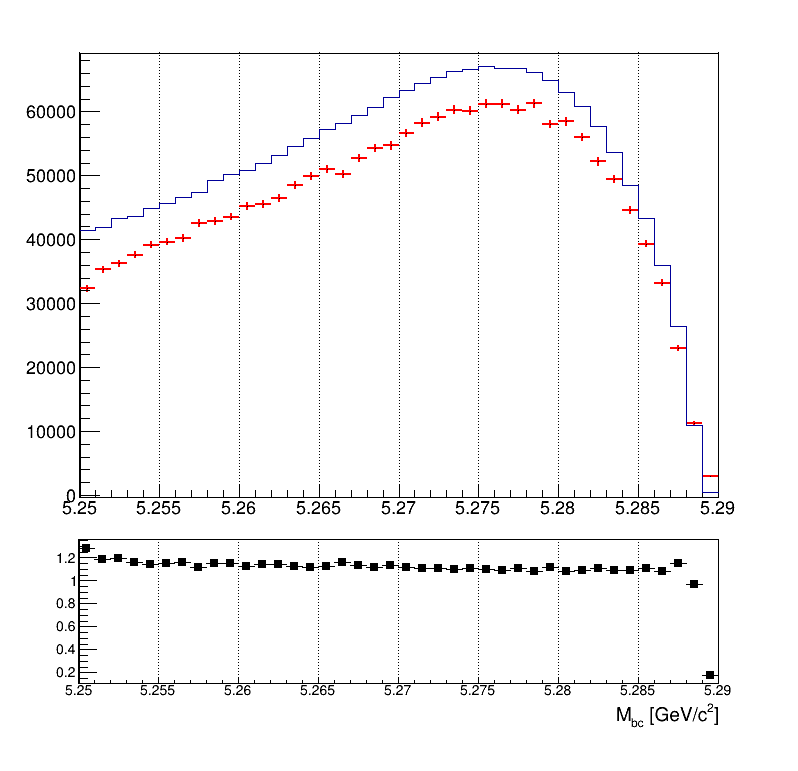
\includegraphics[width=.45\textwidth]{06-chargedAnticorrBtoLambda/figs/on_scaled_offRes_stream0_continuum.png}}
\subcaptionbox{\label{fig:stream1_chargedB_anticorrLambdaCoffresonance_scaled_check}}
{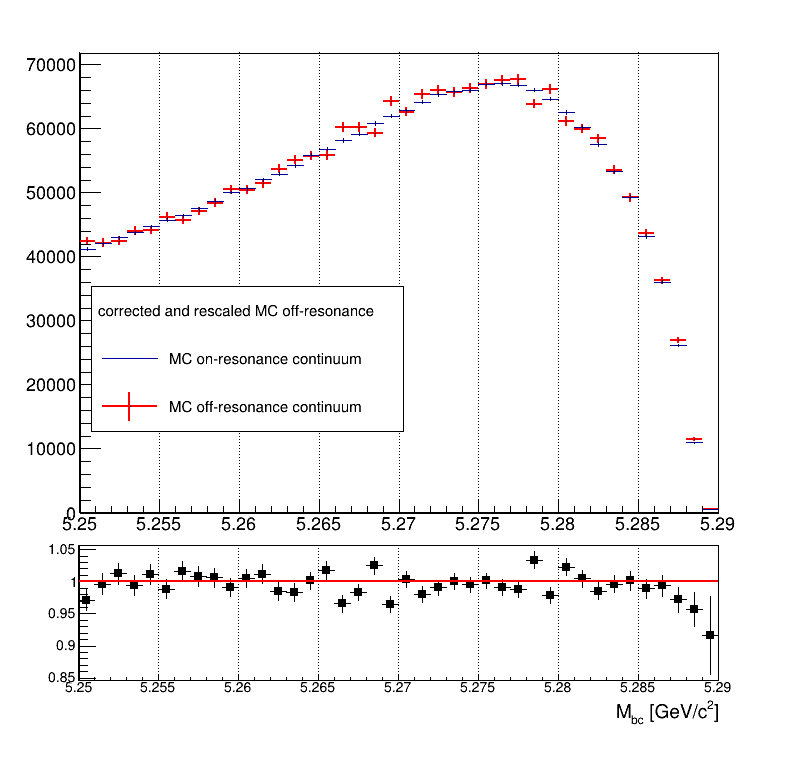
\includegraphics[width=.44\textwidth]{06-chargedAnticorrBtoLambda/figs/stream1_chargedB_anticorrLambdaCoffresonance_scaled_check.png}} 
\caption{On the left: $M_{bc}$ distributions of the MC off-resonance sample and the MC continuum sample with applied continuum suppression. On the right: $M_{bc}$ distributions of the corrected scaled MC off-resonance and on-resonance MC continuum.}
\end{figure}


\newpage
\subsection{ $B_{tag}$ fit}\label{sec:chargedAnticorrBtagFit}


\begin{figure}[h!]
\centering
{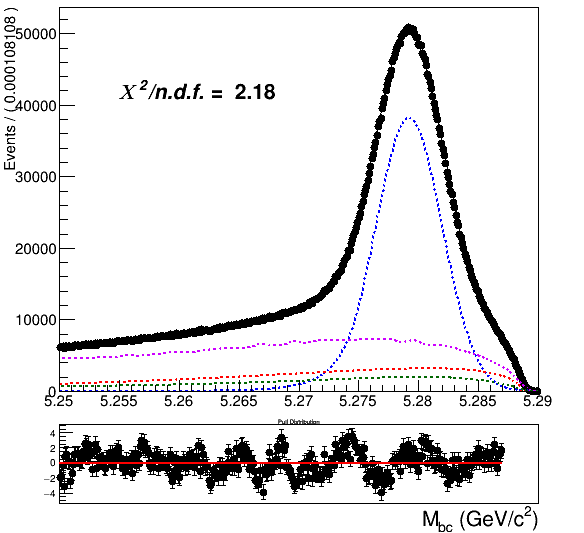
\includegraphics[width=0.50\textwidth]{06-chargedAnticorrBtoLambda/figs/stream1_chargedBtag_Total_fit_sigmaCB_misRecoSlope_free_370bins.png}}
\caption{Total fit of tagged $B$ mesons on Monte Carlo simulated data.}
\label{fig:chargedAnticorrLambdaC_BtagFit}
\end{figure}
\vspace{1.5cm} 

An independent Monte Carlo stream was used to test the total fit model on tagged $B$ meson candidates.
As in the 2D fit, the parameter for the width, $\sigma_{CB}$, of the Crystal Ball is floated and the ratio between expected crossfeed background events and  misreconstructed signal events is fixed from the MC. 
The Argus function describing the misreconstructed signal is also not fully constrained: the parameter describing the tail is free.
As in the previous $B_{tag}$ fits, the range for the fit is restricted to values betweeen 5.250 and 5.287 GeV/c$^2$.
Yields for the reconstructed and misreconstructed signal are obtained from the fit:\\
\vspace{0.25 cm}

\begin{tabular}{ |p{2.5cm}||p{4.2cm}|  }
 \hline
 NrecSig  & 2.5099$\cdot$10$^6 \pm$ 4408\\
 NmisSig &  7.82307$\cdot$10$^5 \pm$ 2936 \\
 \hline
\end{tabular}


\vspace{0.5 cm}
\noindent The Total Signal (the sum  NrecSig+NmisSig) is 3292168 $\pm$ 2423 (to be compared with 3299629 from the Monte Carlo), which means a $\sim 3\sigma$ underestimation. As in the case of charged flavor-correlated decays, this can produce some systematic effect which needs to be taken into account.
In fact, a slight underestimation of the Total Signal is found also in the result of the toy Monte Carlo study\footnote{as usual performed with  $3\times10^3$ pseudo-datasets}: \cref{fig:Total_Signal_chargedBtagToyMCstudy} shows the results for the Total Signal events and one can notice a mean value for the pulls consistently below zero.



\begin{figure}[H]
\centering
{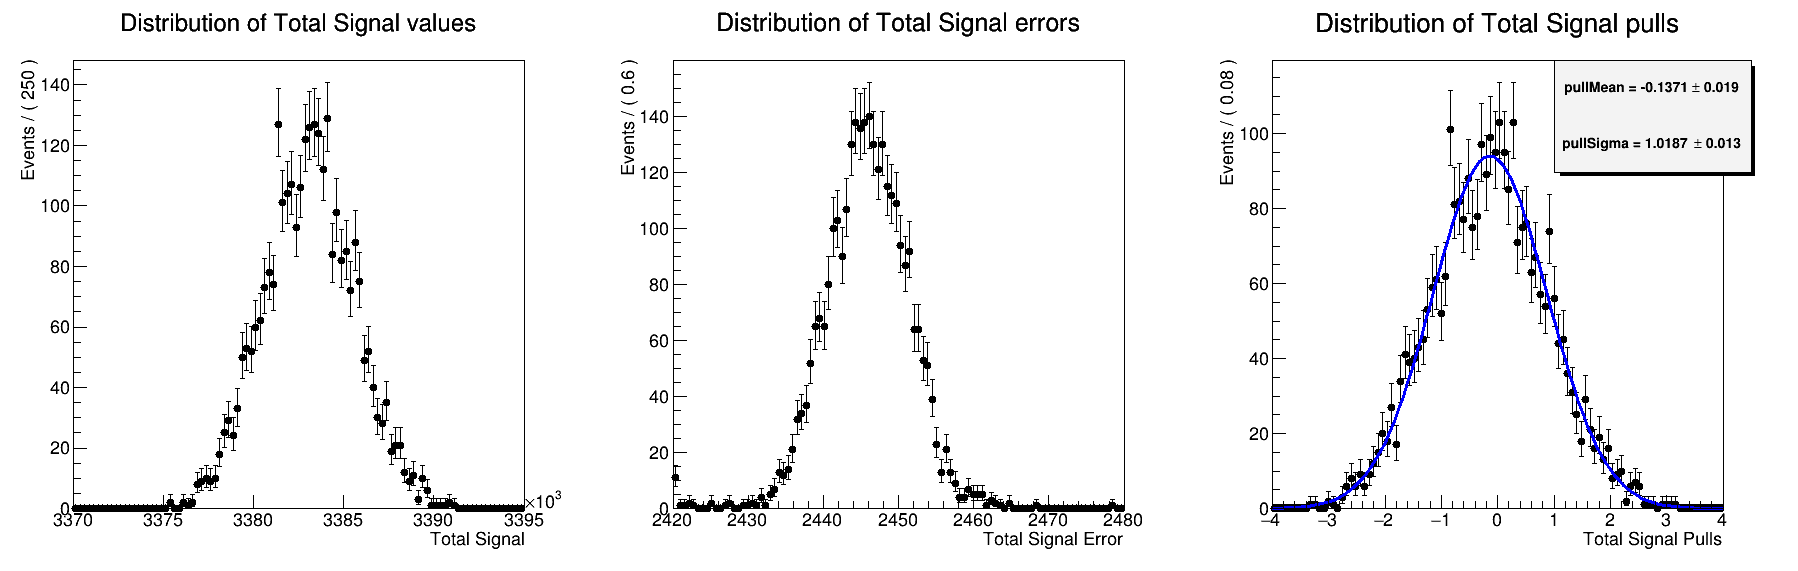
\includegraphics[width=1.\textwidth]{06-chargedAnticorrBtoLambda/figs/Total_Signal_chargedBtagToyMCstudy.png}}
\caption{Toy MC fits of pseudo-data showing the Total Signal yield (left), Total Signal yield errors (center) and the pull distribution of the Total Signal (right).}
\label{fig:Total_Signal_chargedBtagToyMCstudy}
\end{figure}


\subsection{$\Lambda_c$ and FEI efficiency}

The efficiency in reconstructing the ${\Lambda_c}$ baryon after correctly tagging the charged $B$ meson, is as usual estimated as the ratio: 

\begin{equation}
    \frac{N_{recSig}(B_{tag}, \Lambda_c)}{N_{recSig}(B_{tag}^{sig})}
\end{equation}

\vspace{0.5cm}

\noindent where $N_{recSig}(B_{tag}, \Lambda_c))$ are the yields of reconstructed signal from the two dimensional fits (reported in Table \ref{tab:SixStreams_chargedAnticorrLam2Dfits} ) and  $N_{recSig}(B_{tag}^{sig})$ are the yields of correctly reconstructed signal in a fit of $B$ mesons tagged in events where one of the two mesons decayed hadronically and inclusively into a ${\Lambda_c}$ baryon (see Fig \ref{fig:sixstreams_chargedBtagSignal_fit}). This ratio was calculated upon six streams of Monte Carlo simulated data.

\begin{figure}[h!]
\centering
{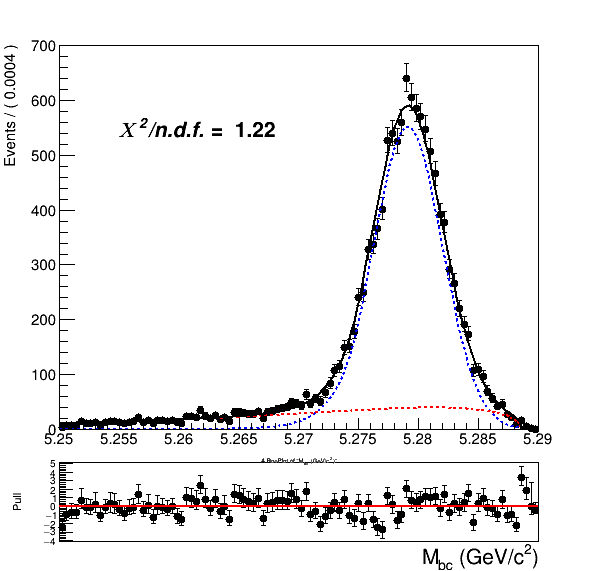
\includegraphics[width=0.40\textwidth]{06-chargedAnticorrBtoLambda/figs/chargedBtag_anticorrLambdaC_TotalSignalBtag_fit.png}}
\caption{Fit of tagged $B$ mesons in the "signal events" sample}
\label{fig:chargedBtag_anticorrLambdaC_TotalSignalBtag_fit}
\end{figure}


\vspace{0.5 cm}
From this and the results listed in \cref{sec:chargedAnticorr2DtotalFit} 
the efficiency to reconstruct ${\Lambda_c}$ is obtained : \\

$\epsilon_{\Lambda_c} = \frac{NrecSig(B_{tag}, \Lambda_c) }{NrecSig(N_{recSig}(B_{tag}} = 40.95 \pm 1.77 \%$  %\hspace{1cm} (KID efficiency corrected value for data: 38.2 $\%$)
\vspace{0.2 cm}

The yields from the fit shown in  Fig. \ref{fig:chargedBtag_anticorrLambdaC_TotalSignalBtag_fit}) are then used to calculate the FEI tag-side efficiency for signal events. The yields from the fit of charged $B_{tag}$ shown in Fig. \ref{fig:stream0_anticorr_chargedBtag_Total_Signal_fit} can be used to calculate the hadronic tag-side efficiency in the generic $B^+B^-$ events case.

The ratio between the two efficiencies is calculated: 
 $\frac{\epsilon^{+}_{FEI,  sig}}{\epsilon^{+}_{FEI}} = 0.973 \pm 0.009 $ \\\vspace{0.4 cm}


\subsection{Studies of Systematic Effects}

The systematic uncertainties are estimated the same way as in the case of charged flavor-correlated decays (see \cref{sec:chargedCorr_continuumBkgSys} and the following Sections).
In Table \ref{tab:systematics_ChargedAnticorr} the systematic uncertainties of the various considered sources are summarized.
Their individual calculation is outlined in the subsequent subsections (the uncertainties on the PID   efficiency corrections are the same already discussed in \cref{sec:chargedCorrPIDcorrSys})

\begin{table}[h]
\centering
\resizebox{0.5\textwidth}{!}{%
\begin{tabular}{lS}
\hline
source              & $\%$  \\
\hline
Continuum modeling      &  0.04 \\
Crossfeed PDFs      &  0.01 \\
Crossfeed fraction      &  0.01 \\
2DFit crossfeed normalization & 0.01 \\
2DFit crossfeed peaking fraction & 0.08* \\
$\epsilon^{+}_{FEI,  sig}/\epsilon^{+}_{FEI}$ & 0.01 \\
$\epsilon_{\Lambda_c}$ & 0.05 \\
Fit bias        & 0.05 \\
PID  &  0.02 \\
Tracking efficiency  & 0.01 \\
\hline
Total                         &   0.12   \\
\hline
\end{tabular}%
}%
\caption{Systematic uncertainties in the determination of the  $B^- \rightarrow \bar{\Lambda}_c^- X$ branching fractions in \si{\percent}.}
\label{tab:systematics_ChargedAnticorr}
\end{table}


* as in the case of charged flavor-correlated decays this uncertainty can be possibly reduced with a new measurement of $B^0 \rightarrow \Lambda_c$ decays.


\subsection{Continuum background modeling}

%, to estimate the systematic uncertainty deriving from statistical uncertainties two-dimensional fits were performed where the parameters' values have been varied by their uncertainties (once with $+$err and then with $-$err). Whereas the impact of statistical uncertainties in the case of the $B_{tag}$ was estimated varying the nominal number of events described with the histogram PDF by Poissonian variation. 
Exemplary, fits used to estimate the impact of these uncertainties deriving from statistical uncertainties are shown here in Figures \ref{fig:Signal_window_Total_2DFit_stream5_chargedAnticorrLambdaC_MinusNcontinuum} - \ref{fig:stream1_chargedBtag_AnticorrTotal_fit_ContinuumSys_Plus}.
Mean deviation values are then obtained for both the two-dimensional fit and the $B_{tag}$ fit.

\begin{tabular}{ |p{2.5cm}||p{2cm}| p{2cm}|  p{2cm}|}
\hline
    Fit    &  $- \sigma$ &  $+ \sigma$ & $ \pm \bar{\sigma}$\\
 \hline
 2D        &     21  & 22  & 22 \\
 $B_{tag}$ &  5800 &  5800 & 5800 \\
 \hline
\end{tabular}

\begin{figure}[H]
\centering
{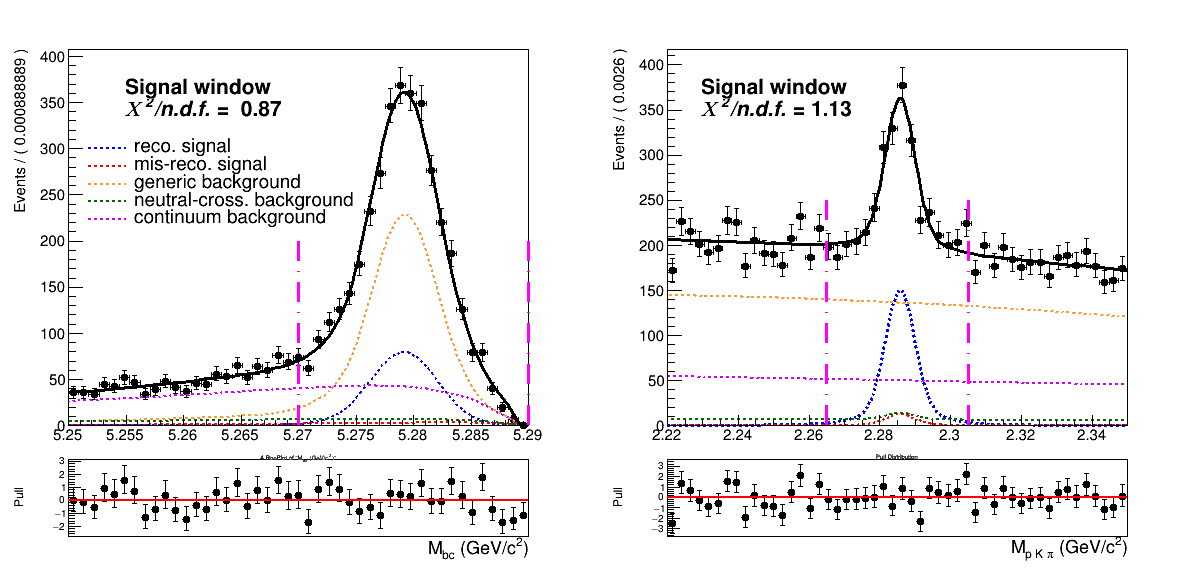
\includegraphics[width=0.85\textwidth]{06-chargedAnticorrBtoLambda/figs/Signal_window_Total_2DFit_stream5_chargedAnticorrLambdaC_MinusNcontinuum.png}}
\caption{Signal window projections of a two dimensional fit on Monte Carlo simulated data where the shaping parameters were varied of their uncertainties.}
\label{fig:Signal_window_Total_2DFit_stream5_chargedAnticorrLambdaC_MinusNcontinuum}
\end{figure}

\begin{figure}[H]
\centering
{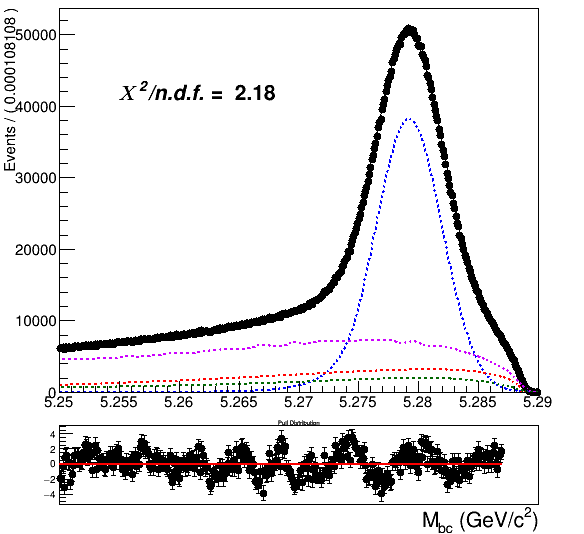
\includegraphics[width=0.5\textwidth]{06-chargedAnticorrBtoLambda/figs/stream1_chargedBtag_AnticorrTotal_fit_ContinuumSys_Plus.png}}
\caption{Fit of tagged $B$ meson candidates on Monte Carlo simulated data where the shaping parameters were varied of their uncertainties.}
\label{fig:stream1_chargedBtag_AnticorrTotal_fit_ContinuumSys_Plus}
\end{figure}




\vspace{0.5 cm}
The estimated systematic uncertainty on Br value from this source is 0.04$\%$.

The continuum suppression cut is found to reject about 68$\%$ of the continuum background in data, whereas it rejects 64$\%$ of the continuum background in MC (66.5$\%$ in on-resonance MC). This means that in data one can expect about 1.4$\%$ less continuum background events. The statistical uncertainty on this fraction of events can be also be taken into account as systematics. But again, as already seen in the case of charged flavor-correlated decays, the statistical uncertainty on the on-resonance continuum background events in MC originates a much larger systematic uncertainty: the relative systematic uncertainty deriving from the different impact on data of the continuum suppression would account for just 0.004$\%$ on the BR value (one order of magnitude smaller than systematics deriving from the statistical uncertainties). This second source is again consequently neglected.

\subsection{Crossfeed background modeling}

This source of systematic uncertainty is again estimated performing the fits varying the parameters of the Crossfeed PDFs  by their uncertainties (see the table below for the deviations in terms of signal yields). 
The resulting absolute systematic uncertainty is about 0.006$\%$ on the BR value, which is rounded up to 0.01$\%$.

 \vspace{0.25 cm}
\begin{table}[H]
\begin{tabular}{ |p{2.5cm}||p{2cm}| p{2cm}|  p{2cm}|}
\hline
    Fit    &  $- \sigma$ &  $+ \sigma$ & $ \pm \bar{\sigma}$\\
 \hline
 2D        &     3  & 3  & 3 \\
 $B_{tag}$ &  1500 &  1100 & 1300 \\
 \hline
\end{tabular}
\caption{Offsets on the signal yields obtained varying the parameters of crossfeed background PDFs within their uncertainties in the two dimensional and $B_{tag}$ fit and mean deviations reported in the last column.}
\end{table}
 \vspace{0.25 cm}

 


\subsection{Crossfeed ratio}

As already done for the charged flavor-correlated decays, the systematic uncertainty on the crossfeed/misreconstructed signal "probability ratio" for the 2D fit 
and crossfeed/misreconstructed ratio is studied  considering a maximal discrepancy up to 20$\%$ between Monte Carlo and data (the procedure adopted is the same as illustrated in \cref{sec:chargedCorrCrossfeedSys}).   


\vspace{0.25 cm}
\begin{table}[H]
\begin{tabular}{ |p{2.5cm}||p{2cm}| p{2cm}|  p{2cm}|}
\hline
    Fit    &  $- \sigma$ &  $+ \sigma$ & $ \pm \bar{\sigma}$\\
 \hline
 2D        &     4  & 8  & 6\\
 $B_{tag}$ &  5800 &  800 & 3300 \\
 \hline
\end{tabular}
\caption{Offsets on the signal yields obtained varying of $\pm$20$\%$ the $k$ ratio in the two dimensional and $B_{tag}$ fit and mean deviations reported in the last column.}
\end{table}
 \vspace{0.25 cm}
The estimated systematic uncertainty on Br value from this source is 0.01$\%$. 
\vspace{0.5 cm}


\subsection{Parametrization of crossfeed normalization in the 2D fit}\label{sec:chargedAnticorrCrossBkgNormalization}

The statistical uncertainties on the parameters used in the  parametrization of crossfeed normalization in  the 2D fit are estimated to originate a systematic uncertainty of 0.01$\%$ on the Br value.


\subsection{Crossfeed peaking fraction in the 2D fit}\label{sec:chargedAnticorrPeakingCrossBkg}

As already done for the charged correlated decays, to estimate this systematic uncertainty the amount of crossfeed events peaking in $M(p K \pi)$  was varied 
in order to cover the uncertainties on the branching fraction for neutral decays and the two-dimensional fit repeated with those values.  The difference in signal yields obtained is reported in the following table. 

\vspace{0.25 cm}
\begin{table}[H]
\begin{tabular}{ |p{2.5cm}||p{2cm}| p{2cm}|  p{2cm}|}
\hline
    Fit    &  $- \sigma$ &  $+ \sigma$ & $ \pm \bar{\sigma}$\\
 \hline
 2D        &     15  & 18  & 16 \\
  \hline
\end{tabular}
\caption{Offsets on the signal yields obtained varying the amount of peaking crossfeed in the $\Lambda_c$ invariant mass and mean deviation.}
\end{table}
 \vspace{0.25 cm}

The uncertainity originated is estimated to be of 0.08$\%$ on the Br value. 

\subsection{Efficiencies}\label{sec:charged_anticorrLam}
 
The ratio between the two FEI efficiencies is: 
 $\frac{\epsilon^{+}_{FEI,  sig}}{\epsilon^{+}_{FEI}} = 0.973 \pm 0.009 $ \\
%\vspace{0.4 cm} 
 The uncertainity on this value originates a systematic uncertainty of 0.01$\%$ on the Br value.
The $\Lambda_c$ reconstruction efficiency is determined to be $\epsilon_{\Lambda_c}$ = 40.95 $\pm 1.77 \%$. When propagating its uncertainty, a systematic error of 0.07$\%$ on the Br value is calculated.

\subsection{Fit biases}

The small bias on the reconstructed signal seen in the two-dimensional fit model produces a not negligible systematic uncertainty on the branching fraction.  The discrepancy in the amount of the total signal estimated by the $B_{tag}$ fit needs to be included as well in the systematic effects.
Propagating the two sources of systematics in the branching fraction calculation results in an additional 0.05$\%$ uncertainty on the branching fraction value.


\subsection{Tracking efficiency}
As for the charged correlated decays, a systematic uncertainty of 0.35$\%$ per track is applied and the total systematic uncertainty is the sum over the 
three charged tracks used to reconstruct the $\Lambda_c$ baryon: 1.05$\%$.
This results in 0.01$\%$ uncertainty on the branching fraction value. 

\subsection{Measured $B^+ \rightarrow {\Lambda_c}^+$ inclusive Branching Fraction}
Using the results from the two dimensional fit reported in \cref{tab:SixStreams_chargedAnticorrLam2Dfits} with all the needed factors known, 
it's possible to examine the agreement between the the branching ratio value used in MC generation and the measured ones. %In \cref{tab:SixStreams_chargedAnticorrLamBR}
As in the charged flavor-correlated decays the average of measured values are about 1$\sigma$ statistical uncertainty away from the average value of the branching ratio set in MC 
(actually already the average value obtained with the total signal fits shows this tendency).  


%\begin{table}[H]   one can first of all notice the slight shift of the branching fraction value obtained with the fits. 
%\centering
%\resizebox{0.95\textwidth}{!}{%
%\setlength{\tabcolsep}{8pt}
%\begin{tabular}{c c c c c c c}
%\toprule
% \hline
%     &  total fit \hspace{0.5 cm}  & signal fit  &  BELLE MC VALUE  \\
% \midrule
% \hline
%stream 0	&	(1.32 $\pm$ 0.12)$\%$  &	(1.19 $\pm$ 0.04)$\%$	 &	(1.233 $\pm$ 0.007)$\%$\\
%stream 1	&	(1.32 $\pm$ 0.11)$\%$	&	(1.26 $\pm$ 0.05)$\%$	 &	(1.218 $\pm$ 0.007)$\%$	\\
%stream 2	&	(1.37 $\pm$ 0.12)$\%$	&	(1.29 $\pm$ 0.05)$\%$	 &	(1.218 $\pm$ 0.007)$\%$\\
%stream 3	&	(1.30 $\pm$ 0.12)$\%$	&	(1.26 $\pm$ 0.05)$\%$	 &	(1.215 $\pm$ 0.007)$\%$\\
%stream 4	&	(1.32 $\pm$ 0.13)$\%$   &	(1.26 $\pm$ 0.05)$\%$	 &	(1.218 $\pm$ 0.007)$\%$\\
%stream 5	&	(1.16 $\pm$ 0.10)$\%$	&	(1.22 $\pm$ 0.05)$\%$	 &	(1.217 $\pm$ 0.007)$\%$\\
%\midrule
%\hline
%average		&	(1.30 $\pm$	0.05)$\%$	&	(1.25 $\pm$	0.02)$\%$	& (1.220 $\pm$ 0.003)$\%$\\
%\bottomrule
%\hline
%\end{tabular}%
%}%
%\caption{Measured branching fraction values obtained using the results listed in \cref{tab:SixStreams_chargedAnticorrLam2Dfits} for the six different streams (only statistical uncertainties are displayed) and its average.}
%\label{tab:SixStreams_chargedCorrLamBR}
%\end{table}



%%%%%%%%%%%%%%%%%%%%%%%%%%%%%%%%%%%%%%%%%%
%%%After parametrization:
%%%%%%%%%%%%%%%%%%%%%%%%%%%%%%%%%%%%%%%%%%
\begin{table}[H]
\centering
\resizebox{0.95\textwidth}{!}{%
\setlength{\tabcolsep}{8pt}
\begin{tabular}{c c c c c c c}

\toprule
 \hline
     &  total fit \hspace{0.5 cm}  & signal fit  &  BELLE MC VALUE  \\
 \midrule
 \hline
stream 0	&	(1.32 $\pm$ 0.11)$\%$  &	(1.19 $\pm$ 0.04)$\%$	 &	(1.233 $\pm$ 0.007)$\%$\\
stream 1	&	(1.32 $\pm$ 0.11)$\%$	&	(1.26 $\pm$ 0.05)$\%$	 &	(1.218 $\pm$ 0.007)$\%$	\\
stream 2	&	(1.37 $\pm$ 0.12)$\%$	&	(1.29 $\pm$ 0.05)$\%$	 &	(1.218 $\pm$ 0.007)$\%$\\
stream 3	&	(1.31 $\pm$ 0.11)$\%$	&	(1.26 $\pm$ 0.05)$\%$	 &	(1.215 $\pm$ 0.007)$\%$\\
stream 4	&	(1.50 $\pm$ 0.12)$\%$   &	(1.26 $\pm$ 0.05)$\%$	 &	(1.218 $\pm$ 0.007)$\%$\\
stream 5	&	(1.12 $\pm$ 0.12)$\%$	&	(1.22 $\pm$ 0.05)$\%$	 &	(1.217 $\pm$ 0.007)$\%$\\
\midrule
\hline
average		&	(1.32 $\pm$	0.05)$\%$	&	(1.25 $\pm$	0.02)$\%$	& (1.220 $\pm$ 0.003)$\%$\\
\bottomrule
\hline
\end{tabular}%
}%
\caption{Measured branching fraction values obtained using the results listed in \cref{tab:SixStreams_chargedAnticorrLam2Dfits} for the six different streams (only statistical uncertainties are displayed) and its average.}
\label{tab:SixStreams_chargedAnticorrLamBR}
\end{table}

\noindent As in the charged flavor-correlated decays the precision obtained on Monte Carlo simulated data is improved by factors compared to the branching fraction measured by BaBar experiment (see  \cite{PhysRevD.75.072002}). 

%charged anticorrelated decays on PDG: $2.1^{+0.9}_{-0.6}\%$
